L'interfaccia grafica è realizzata tramite il framework \glock{Angular}, quindi il design architetturale utilizzato è il \textit{Model View ViewModel} (\textit{MVVM}) che è intrinseco nel framework stesso. \\
La comunicazione con il server avviene tramite \glock{WebSocket} e dunque asincrono. Viene sfruttato il design pattern \textit{Observer} per permettere un'aggiornamento asincrono dei componenti dell'interfaccia.\\
Inoltre, per garantire l'estensibilità del codice, il servizio \textit{WebSocketService} implementa l'interfaccia \textit{ServerService} che mette a disposizione i metodi per interfacciarsi con il server. In questo modo un cambio di tecnologia, ad esempio passando a richieste \glock{Http}; non comporterebbe uno stravolgimento dell'architettura. \\
Per lo stesso motivo sono previste delle interfacce per rappresentare i vari tipi di messaggi che vengono ricevuti dal server, che vengono successivamente implementate per specificarne le caratteristiche. \\
Per garantire che ogni componente riceva solo i dati di suo interesse, vengono utilizzate delle classi definite da utente per rappresentare la trasmissione delle informazioni tra i componenti. \\
Si è pianificato di avere un componente per ogni funzionalità principale che l'interfaccia mette a disposizione all'utente. \\
\newline
Di seguito l'architettura dell'interfaccia viene rappresentata tramite due diagrammi delle classi: il primo per descrivere il \textit{Model}, e quindi le modalità con cui i messaggi vengono inviati e ricevuti dal server, ed il secondo, per il \textit{Viewmodel} che rappresenta la struttura dei vari \glock{Angular Components}. La parte di \textit{View} comprende i templates degli \glock{Angular Components}, e quindi la struttura del codice \glock{HTML}. \\


\newpage

\begin{landscape}
	\begin{figure}[h!]
		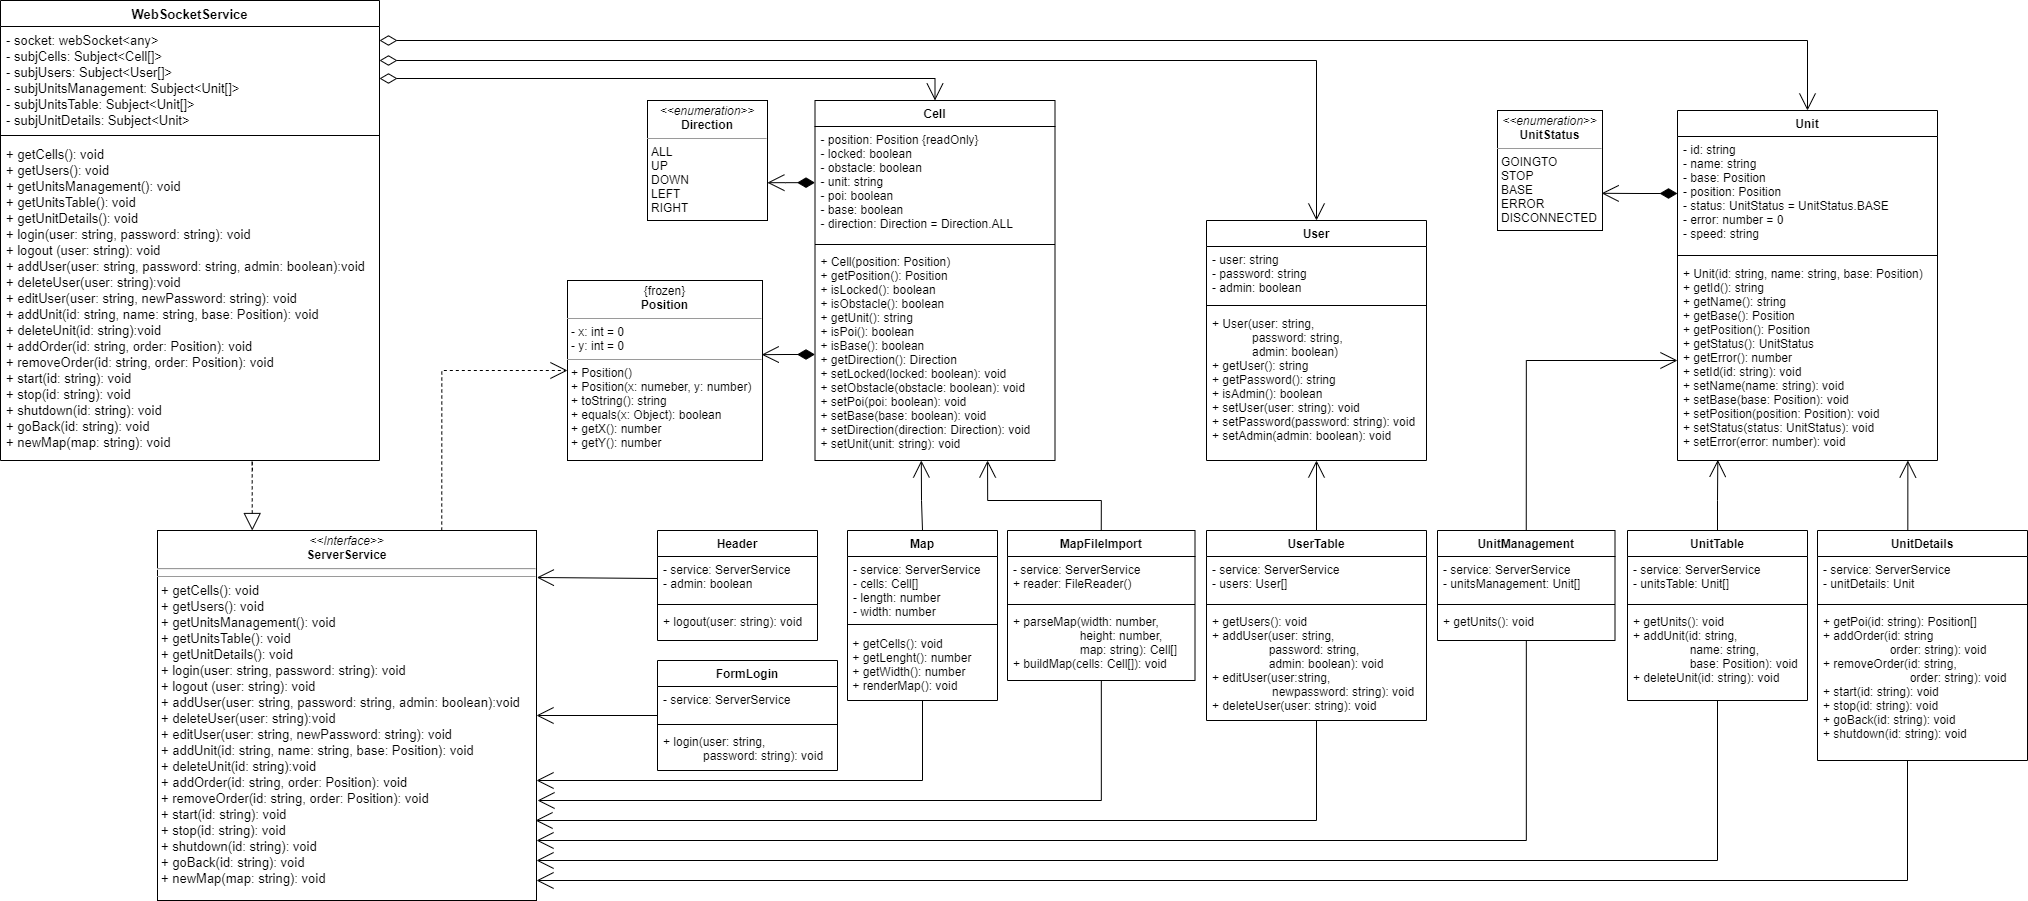
\includegraphics[width=24cm]{img/ui_component.png}
		\caption{Architettura dell'interfaccia - View Model}
	\end{figure}
\end{landscape}
\newpage

\begin{landscape}
	\begin{figure}[h!]
		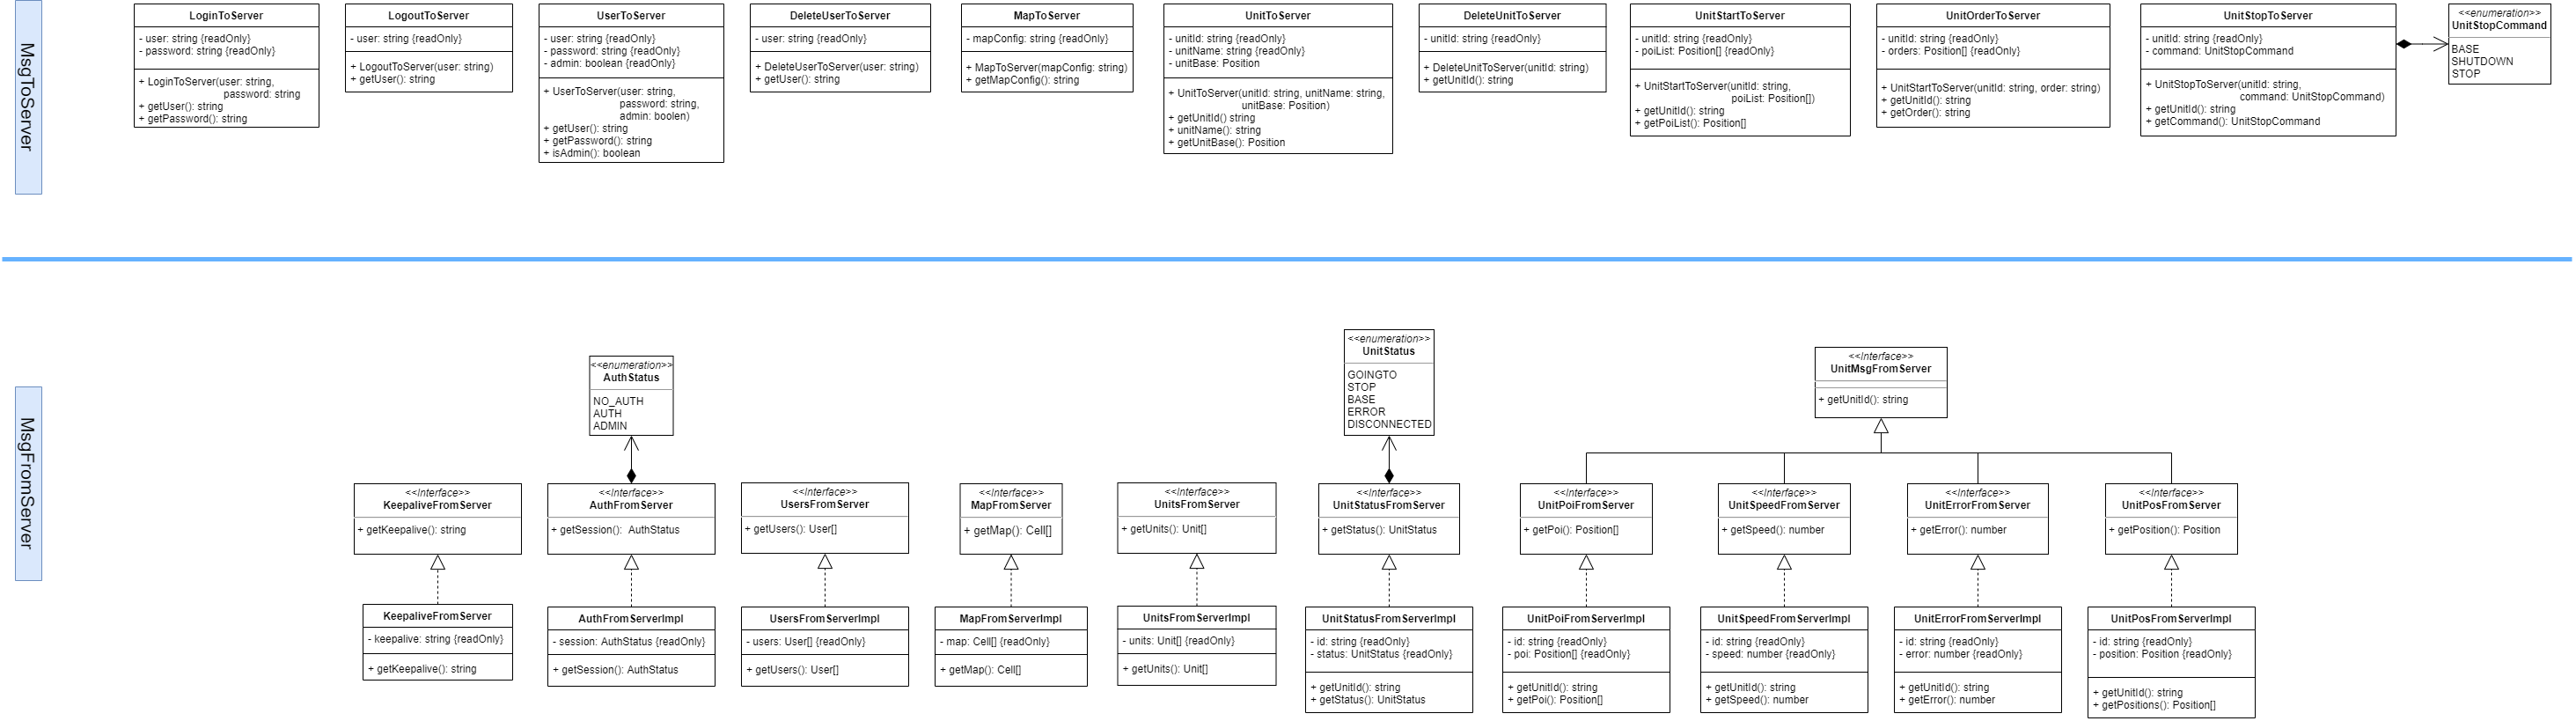
\includegraphics[width=24cm]{img/ui_messaggi.png}
		\caption{Architettura dell'interfaccia - Model}
	\end{figure}
\end{landscape}